\chapter{Caracterización de Conjuntos de Datos}
\label{cap:caracterizacion_datasets}

El presente capítulo tiene como objetivo principal
la caracterización de conjuntos de datos de imágenes médicas de patología digital, esto mediante la 
identificación de variables demográficas y parámetros de adquisición relevantes para el estudio de \textit{bias} 
y \textit{fairness}. 
De esta forma, se realizó una revisión y sistematización de diversos conjuntos de datos públicos de 
\textit{Whole Slide Images}
(WSI), considerando tanto sus atributos clínicos y demográficos como las técnicas bajo las cuales
las imágenes fueron generadas, documentadas y puestas a disposición.

En este contexto, la caracterización de conjuntos de datos no se limita a una descripción catalográfica, sino que 
constituye una etapa analítica necesaria para identificar posibles fuentes de \textit{bias} y \textit{fairness} antes de la evaluación 
de modelos. Sobre esta base, el capítulo examina los conjuntos de datos recopilados, identifica variables comunes 
entre ellos y analiza las condiciones que permiten construir espacios comparables de evaluación, con especial
énfasis en los conjuntos de cáncer de mama y cáncer colorrectal seleccionados para las etapas posteriores 
del trabajo.

\section{Marco de \textit{bias} para la caracterización de los conjuntos de datos}
\label{sec:marco_bias}

La caracterización de los conjuntos de datos se organiza mediante un marco orientado a identificar indicadores observables compatibles con mecanismos de \textit{bias} potencialmente presentes en los datos disponibles. Este marco permite complementar la descripción de los recursos con una interpretación centrada en las condiciones que pueden afectar la representatividad de las cohortes, la comparabilidad entre conjuntos de datos y la interpretación de los resultados experimentales.

El análisis considera tres mecanismos principales: \textit{bias} de representación, \textit{bias} de adquisición y limitaciones de documentación y sesgo de selección. Estos mecanismos se relacionan, respectivamente, con la composición de los subgrupos presentes en las cohortes, con las condiciones técnicas de generación de las imágenes y con el nivel de disponibilidad y calidad de los metadatos, así como con los criterios que determinan qué casos ingresan al conjunto de datos o a la cohorte analítica. Cabe señalar que estos mecanismos no son exhaustivos ni mutuamente excluyentes: el capítulo evalúa indicadores observables compatibles con dichos mecanismos, sin establecer una relación causal directa entre la presencia de un indicador y la aparición de una brecha de \textit{fairness} en un modelo entrenado con estos datos.

La identificación de un mecanismo potencial de \textit{bias} no implica, por sí sola, que un conjunto de datos sea inadecuado para su utilización experimental. Su relevancia radica en que proporciona antecedentes para contextualizar diferencias entre cohortes y para interpretar, con la cautela necesaria, posibles disparidades de desempeño entre subgrupos o escenarios de evaluación.

La tipología adoptada no pretende ser original ni exhaustiva, sino operativa: constituye una adaptación, restringida a las fuentes observables en los recursos disponibles, de taxonomías previamente establecidas en la literatura. \textcite{suresh2021framework} proponen un marco que identifica siete fuentes distintas de daño a lo largo del ciclo de vida de un sistema de aprendizaje automático, diferenciando entre las que se originan en la generación de los datos, sesgo histórico, de representación y de medición, y las que emergen en las etapas de desarrollo, evaluación y despliegue. Por su parte, \textcite{mehrabi2021survey} sistematizan las fuentes de \textit{bias} según se originen en los datos o en los algoritmos, y las vinculan con las definiciones formales de \textit{fairness} utilizadas para su medición. Los tres mecanismos considerados en este capítulo se sitúan íntegramente en el primer grupo de ambas taxonomías, esto es, en las fuentes atribuibles a la procedencia y construcción de los datos: el \textit{bias} de representación corresponde al sesgo de representación en el sentido de \textcite{suresh2021framework}; el \textit{bias} de adquisición constituye una forma de sesgo de medición asociada al instrumento de digitalización; y las limitaciones de documentación y el sesgo de selección determinan qué población queda efectivamente representada en la cohorte analítica. Las fuentes de \textit{bias} originadas en el modelo, en la función de pérdida o en el procedimiento de evaluación quedan explícitamente fuera del alcance de este capítulo y se abordan en los Capítulos~\ref{cap:seleccion_modelos}~y~\ref{cap:evaluacion_modelos}.

\subsection{Mecanismos de \textit{bias} considerados}

El primer mecanismo corresponde al \textit{bias} de representación. Este se refiere a la distribución desigual de subgrupos demográficos dentro de una cohorte o entre cohortes comparables. En este estudio, dicho mecanismo se examina principalmente mediante las variables edad y sexo, debido a su utilidad para la posterior estratificación del desempeño por subgrupos. La subrepresentación de determinados grupos puede limitar la estabilidad de las estimaciones y contribuir a disparidades de rendimiento en sistemas de patología computacional \parencite{vaidya2024demographic}.

De manera complementaria, se analiza la distribución de las variables objetivo de cada dominio: HER2 y subtipo molecular en cáncer de mama, y sitio anatómico y lateralidad en cáncer colorrectal. Estas variables no se interpretan como atributos sensibles, sino como indicadores de desbalance de clases, diferencias de prevalencia y heterogeneidad clínica entre cohortes. Su análisis permite determinar si las tareas definidas dentro de cada dominio se sustentan en categorías suficientemente representadas y comparables entre conjuntos de datos.

El segundo mecanismo corresponde al \textit{bias} de adquisición. Este mecanismo se asocia a las diferencias técnicas involucradas en la generación y digitalización de las imágenes histopatológicas. Entre los factores de interés se encuentran el escáner utilizado, el período de adquisición, la magnificación y la tinción. Tales condiciones pueden producir variaciones sistemáticas en la apariencia visual de las imágenes, incluso cuando los casos pertenecen a un mismo dominio clínico.

La relevancia de este mecanismo se sustenta en la posibilidad de que las imágenes contengan señales asociadas a su procedencia o a sus condiciones de adquisición. En particular, se ha demostrado que el sitio de adquisición puede ser inferido a partir de imágenes histopatológicas digitalizadas, lo que evidencia que los modelos pueden acceder a patrones técnicos ajenos a la morfología de interés \parencite{alsaafin2023biased}. Por ello, la heterogeneidad de adquisición se considera una fuente potencial de correlaciones espurias entre características visuales, procedencia institucional y etiquetas clínicas.

Este tipo de correlación espuria corresponde, en la literatura de aprendizaje profundo, al fenómeno denominado \textit{shortcut learning}: reglas de decisión que alcanzan un desempeño elevado en los conjuntos de evaluación habituales pero que fallan al transferirse a condiciones de prueba más exigentes, porque el modelo explota atributos superficiales correlacionados con la etiqueta en lugar de la estructura de interés \parencite{geirhos2020shortcut}. En el contexto de la imagen médica, se ha mostrado que estos atajos pueden asociarse a atributos demográficos y traducirse en disparidades de desempeño entre subgrupos, lo que los vincula directamente con la evaluación de \textit{fairness} \parencite{brown2023shortcut}. De manera complementaria, las diferencias sistemáticas entre las distribuciones de imágenes de distintas cohortes constituyen un caso de \textit{domain shift}, fenómeno que en patología digital se manifiesta como discrepancias entre \textit{whole-slide images} introducidas, entre otros factores, por diferencias en el \textit{pipeline} de adquisición entre centros médicos o a lo largo del tiempo \parencite{stacke2021domainshift}.

La relación entre ambos conceptos y el marco adoptado en este capítulo es la siguiente: el \textit{bias} de adquisición es el \textbf{mecanismo de origen} observable en los metadatos; el \textit{domain shift} es la \textbf{manifestación distribucional} de dicho mecanismo sobre las representaciones de imagen; y el \textit{shortcut learning} es el \textbf{modo de falla} por el cual esa heterogeneidad podría traducirse en disparidades de desempeño. Esta cadena describe un riesgo potencial, no un resultado: el presente capítulo documenta únicamente los indicadores observables del primer eslabón, la asociación entre conjunto de datos y condiciones técnicas de adquisición (Sección~\ref{sec:adquisicion}), mientras que la verificación empírica de los dos siguientes requiere entrenar y evaluar modelos, y se aborda en los Capítulos~\ref{cap:seleccion_modelos}~y~\ref{cap:evaluacion_modelos}.

El tercer mecanismo agrupa dos fenómenos: las limitaciones de documentación y el sesgo de selección. Las limitaciones de documentación se refieren a la ausencia o insuficiencia de metadatos que impiden observar o auditar una fuente de \textit{bias}. Entre ellas se encuentran la falta de reporte de variables demográficas, la ausencia de parámetros de adquisición, la codificación incompleta de diagnósticos y la falta de trazabilidad entre casos, imágenes y metadatos. El sesgo de selección, por su parte, se refiere a los criterios explícitos o implícitos, que determinan qué casos ingresan al conjunto de datos original o, posteriormente, a la cohorte analítica de una tarea específica.

En términos operativos, las limitaciones de documentación se examinan mediante la disponibilidad de variables demográficas, clínicas y técnicas, la proporción de valores faltantes y la completitud agregada, reportadas en las Tablas~\ref{tab:dataset_global_summary}~y~\ref{tab:completitud_agregada}, y en la Tabla~\ref{tab:missingness_top_variables} del Apéndice~\ref{appendix:tablasdatasets}. El sesgo de selección se examina mediante la trazabilidad de muestras a lo largo del pipeline de datos: desde el registro original hasta la cohorte analítica de cada tarea, incluyendo las pérdidas por falta de etiqueta, falta de atributo sensible o ausencia de imagen digitalizada. Esta trazabilidad se presenta en la Sección~\ref{sec:trazabilidad_muestras}. Una documentación insuficiente restringe la posibilidad de determinar si los subgrupos se encuentran adecuadamente representados o si las condiciones de adquisición pueden introducir fuentes de variación no controladas \parencite{galanty2024}.

Los mecanismos descritos pueden presentarse simultáneamente. Por ejemplo, una cohorte puede concentrar sus casos en determinados grupos etarios, haber sido digitalizada mediante un único escáner y, al mismo tiempo, presentar una cobertura incompleta de variables clínicas o moleculares. En consecuencia, la interpretación de cada conjunto de datos requiere considerar conjuntamente su composición poblacional, sus condiciones de adquisición y la calidad de su documentación.

\subsection{Relación entre mecanismos de \textit{bias} y variables observables}

La Tabla~\ref{tab:mecanismos_bias_variables} presenta la relación entre los mecanismos de \textit{bias} considerados y las variables o indicadores observables disponibles en las tablas de caracterización presentadas a lo largo del capítulo. Esta relación establece una pauta para interpretar la evidencia obtenida durante la caracterización de los conjuntos de datos.

\begin{table}[H]
\centering
\caption{Relación entre mecanismos de \textit{bias}, variables observables y fenómeno teórico asociado en los conjuntos de datos analizados.}
\label{tab:mecanismos_bias_variables}
\small
\begin{tabular}{p{2.6cm} p{4.8cm} p{4.8cm}}
\hline
\textbf{Mecanismo de \textit{bias}} &
\textbf{Variables o indicadores observables} &
\textbf{Fenómeno teórico asociado} \\
\hline

\textit{Bias} de representación &
Edad, sexo y distribución de categorías clínicas, anatómicas, diagnósticas o moleculares. &
Sesgo de representación \parencite{suresh2021framework}; estimaciones inestables en subgrupos de baja frecuencia. \\
\hline

\textit{Bias} de adquisición &
Escáner, período de adquisición, magnificación, tinción y modalidades de imagen reportadas. &
\textit{Domain shift} entre cohortes \parencite{stacke2021domainshift}; riesgo potencial de \textit{shortcut learning} sobre firmas técnicas \parencite{geirhos2020shortcut,howard2021site}. \\
\hline

Limitaciones de documentación y sesgo de selección &
Disponibilidad de metadatos, valores faltantes, completitud agregada, trazabilidad de muestras desde el registro original hasta la cohorte analítica y criterios de inclusión/exclusión en cada etapa del pipeline. &
Sesgo de selección y no observabilidad del sesgo; imposibilidad de auditar fuentes de \textit{bias} no documentadas \parencite{suresh2021framework}. \\
\hline
\end{tabular}
\end{table}

La relación entre mecanismos y variables observables no busca atribuir automáticamente toda diferencia entre cohortes a una fuente de \textit{bias}. Su finalidad es proporcionar un criterio sistemático para identificar qué diferencias pueden reflejar desbalances de representación, heterogeneidad técnica o restricciones en la documentación y selección. La tercera columna indica el fenómeno que la literatura asocia a cada mecanismo; su inclusión tiene un propósito interpretativo y no implica que dicho fenómeno haya sido verificado empíricamente en los conjuntos de datos analizados. De este modo, la caracterización descriptiva permite establecer condiciones de comparabilidad entre cohortes y reconocer fuentes de variación que deben ser consideradas al interpretar el comportamiento de los modelos. La aplicación cuantitativa de esta pauta sobre las cohortes curadas y las cohortes analíticas por tarea se presenta en la Sección~\ref{sec:analisis_cuantitativo_bias}.

\section{Descripción global de los conjuntos de datos}

Con el fin de establecer una base empírica para el estudio de \textit{bias} y \textit{fairness} en patología digital, se realizó una revisión bibliográfica estructurada de conjuntos de datos públicos de imágenes histopatológicas digitales. La selección de estos recursos respondió a su relevancia dentro del dominio de las \textit{Whole Slide Images} (WSI), a la disponibilidad de metadatos clínicos y demográficos, y a su potencial utilidad para tareas de clasificación, predicción pronóstica, análisis multimodal y evaluación de modelos fundacionales.

En su conjunto, los conjuntos de datos recopilados cubren distintos órganos, escenarios clínicos, escalas de tamaño y niveles de documentación, lo que permite observar de manera temprana la heterogeneidad estructural que caracteriza a este campo. Los conjuntos considerados corresponden a NDB-UFES \parencite{NDBUFES2023}, \textit{The Digital Brain Tumour Atlas} \parencite{DigitalBrainTumourAtlas2022}, HISTAI \parencite{HISTAI2025}, SOPHIE \parencite{SOPHIE2023}, BCNB \parencite{BCNB2021}, CLWD \parencite{CLWD2026}, SurGen \parencite{SurGen2026}, \textit{Ovarian Bevacizumab Response} \parencite{OvarianBevacizumab2022} e \textit{Histology HSI-BC-Recurrence} \parencite{HistologyHSIBCRecurrence2025}. En términos generales, estos recursos abarcan dominios como cáncer oral, tumores cerebrales, cáncer de mama, adenocarcinoma pulmonar, cáncer colorrectal, neoplasias melanocíticas spitzoides y cáncer de ovario.

\paragraph{Nota metodológica sobre la unidad analítica.} La revisión comprende nueve conjuntos de datos originales; sin embargo, la unidad analítica utilizada en las tablas de este capítulo no coincide siempre con el recurso publicado. \textit{HISTAI} se desagrega en tres subcohortes independientes (HISTAI-Breast, HISTAI-CRC-B1 e HISTAI-CRC-B2) por presentar dominios clínicos repetidos con otros recursos de la revisión, mientras que \textit{SurGen} se mantiene como un único conjunto de datos pese a integrar dos lotes (SR386 y SR1482). En consecuencia, las tablas de este capítulo distinguen nueve recursos originales de once unidades analíticas; la justificación de ambas decisiones se presenta en la Sección~\ref{sec:nota_unificacion_surgen}.

A continuación, se presenta una descripción individual de cada uno de los conjuntos de datos considerados en esta revisión, resumiendo su foco clínico, su escala y su desenlace en la preselección. La síntesis de las características esenciales de los recursos y de su desenlace en la preselección se presenta en la Tabla~\ref{tab:resumen_datasets_global} del Apéndice~\ref{appendix:tablasdatasets}, junto con el detalle de los parámetros reportados por cada conjunto de datos.

Se revisaron nueve recursos públicos de patología digital con dominios, escalas, completitud y niveles de documentación heterogéneos. La Tabla~\ref{tab:resumen_datasets_global} sintetiza su propósito, variables disponibles y desenlace de la preselección; la Tabla~\ref{tab:acquisition-all-datasets} resume las condiciones de adquisición documentadas. Esta revisión permitió identificar mama y colorrectal como los únicos dominios con cohortes repetidas y variables comparables suficientes para la evaluación posterior.

La Tabla \ref{tab:acquisition-all-datasets} muestra los parámetros de adquisición reportados por cada recurso, con el fin de identificar posibles fuentes de variabilidad técnica entre cohortes. En particular, se consideraron el período de adquisición, el escáner utilizado, la magnificación, la tinción y la presencia de modalidades complementarias cuando tales antecedentes estaban explícitamente documentados. Esta síntesis permite complementar la caracterización global de los conjuntos de datos y hacer visible qué tan trazables son sus condiciones de adquisición para análisis posteriores de \textit{bias} y \textit{fairness}.

\begin{table}[htbp]
\centering
\caption{Parámetros de adquisición reportados en los datasets revisados}
\label{tab:acquisition-all-datasets}
\renewcommand{\arraystretch}{1.15}
\resizebox{\textwidth}{!}{%
\begin{tabular}{p{3.2cm} p{3.0cm} p{3.4cm} p{2.6cm} p{2.8cm}}
\hline
\textbf{Dataset} & \textbf{Scanner} & \textbf{Período de adquisición} & \textbf{Magnificación} & \textbf{Tinción} \\
\hline
NDB-UFES &
Olympus DP73 &
2011--2021 &
10x y 40x &
H\&E \\
The Digital Brain Tumour Atlas &
Hamamatsu NanoZoomer 2.0 HT &
1995--2019 &
40x &
H\&E \\
HISTAI &
Leica Aperio GT450 y AT2; algunos Hamamatsu y 3DHISTECH &
No reportado &
20x; fracción a 40x &
H\&E mayoría \\
SOPHIE &
Ventana iScan HT (Roche) &
1988--2020 &
40x  &
H\&E \\
BCNB &
No reportado &
No reportado &
20x &
H\&E \\
CLWD &
SQS-600P &
2020--2023 &
80x  &
H\&E \\
SurGen &
ZEISS AxioScan.Z1 &
No reportado &
40x  &
H\&E \\
Ovarian Bevacizumab Response &
Leica AT Turbo (Leica, Germany) &
No reportado &
20x &
H\&E \\
Histology HSI-BC-Recurrence &
Pannoramic 250 Flash III (3DHISTECH Ltd.) &
2006--2015 &
20x &
H\&E \\
\hline
\end{tabular}%
}
\end{table}

\section{Metodología de caracterización descriptiva}

Con el objetivo de caracterizar de manera homogénea los conjuntos de datos descritos en la sección anterior, se desarrolló un \textit{script} de Python denominado \textit{DatasetAnalyzer}, diseñado para procesar automáticamente los metadatos tabulares de cada recurso y generar resúmenes estadísticos y visualizaciones descriptivas. Esta etapa tuvo un propósito principalmente metodológico: describir de forma sistemática qué variables estaban disponibles, cómo se distribuían y qué nivel de completitud presentaban, construyendo una base homogénea de caracterización útil para los análisis posteriores de \textit{bias} y \textit{fairness}. El uso de un procedimiento automatizado fue necesario debido a la heterogeneidad de los conjuntos revisados, tanto en dominios clínicos como en nomenclatura de columnas, codificación y estructuración de metadatos, lo que habría hecho poco escalable y reproducible una inspección manual caso a caso.

La caracterización se aplicó de forma transversal a todos los recursos, considerando como unidad de análisis los metadatos de cada conjunto de datos o subcohorte. Esta distinción fue relevante en \textit{SurGen}, tratado como un único conjunto de datos pese a integrar los lotes SR386 y SR1482 (tumores primarios con datos de supervivencia, y casos con sitios metastásicos, respectivamente), dado que ambos proceden del mismo estudio hospitalario (NHS Lothian, Escocia) y comparten estructura de metadatos, protocolo de tinción y condiciones de adquisición; como consecuencia, las variables reportadas únicamente en un lote adquieren \textit{missingness} estructural en el conjunto unificado, y el Apéndice~\ref{appendix:tablasdatasets} conserva la desagregación de los lotes para preservar la trazabilidad original. De manera análoga, la naturaleza multitejido de HISTAI motivó identificar las subcolecciones HISTAI-Breast, HISTAI-CRC-B1 e HISTAI-CRC-B2 como unidades independientes, al presentar dominios clínicos repetidos con otros recursos de la revisión. El \textit{script} fue implementado como una clase configurable que ejecuta una secuencia fija de pasos, carga de datos, estandarización de columnas, normalización de valores faltantes, limpieza de texto, recodificación, conversión de tipos, creación de variables derivadas, detección automática de tipo de columna y generación de reportes y gráficos, aplicable a los nueve conjuntos de datos revisados independientemente de su formato original. Cabe precisar que los metadatos corresponden a la unidad de reporte definida por los autores de cada conjunto de datos, habitualmente un paciente o caso clínico, mientras que un mismo registro puede estar asociado a más de una \textit{slide} digitalizada; la cuantificación de esta relación paciente-\textit{slide} se aborda en capítulos posteriores.

El \textit{script} incorporó operaciones de limpieza y estandarización (normalización de columnas, recodificación de categorías, identificación de valores faltantes) y una tipificación de variables en cinco grupos, numéricas, categóricas, temporales, booleanas y de texto libre, combinando reglas declarativas con detección automática; el detalle de estas reglas y de la cardinalidad observada se presenta en el Apéndice~\ref{appendix:detalles_datasetanalyzer}. En HISTAI, cuyos metadatos clínicos se encontraban mayormente en texto libre, se aplicó sobre las subcohortes una etapa de estructuración semántica que generó variables derivadas comparables (diagnóstico normalizado, grupo taxonómico, lateralidad, sitio anatómico) sin modificar la información de base. El \textit{script} generó, por dataset, un resumen global (registros, variables por tipo, celdas faltantes), reportes de \textit{missingness} por variable, estadísticas numéricas y tablas de frecuencia categóricas, además de salidas exploratorias para identificar columnas poco informativas y distribuciones desbalanceadas. Las visualizaciones descriptivas completas se incluyen en el Apéndice~\ref{appendix:detalles_datasetanalyzer}.

Las Tablas~\ref{tab:dataset_global_summary} y~\ref{tab:completitud_agregada} muestran heterogeneidad relevante en tamaño y completitud: los recursos van desde 47 hasta más de 3.000 registros, y en algunos casos la \textit{missingness} se concentra en pocos atributos específicos (Tabla~\ref{tab:missingness_top_variables} del Apéndice~\ref{appendix:tablasdatasets}), mientras que en otros compromete de forma más transversal la utilidad descriptiva del recurso. CLWD, BCNB y HSI-BC presentan metadatos casi completos, mientras que TDBTA, SurGen y SOPHIE concentran mayor \textit{missingness}; en SurGen, una parte corresponde a ausencia estructural de variables exclusivas de una subcohorte.\label{sec:nota_unificacion_surgen} Estos hallazgos permitieron distinguir entre conjuntos con metadata más completa y recursos cuyo valor analítico dependía de un procesamiento adicional más intensivo, apoyando la toma de decisiones sobre qué conjuntos de datos resultaban más adecuados para las etapas posteriores del estudio.

\begin{table}[htbp]
\centering
\caption{Caracterización global de los conjuntos de datos analizados mediante \textit{DatasetAnalyzer}.}
\label{tab:dataset_global_summary}
\small
\setlength{\tabcolsep}{6pt}
\begin{tabular}{lrrrrrrr}
\toprule
Dataset & Registros & Variables & Num. & Cat. & Fecha & Texto & \textit{Missing} (\%) \\
\midrule
Ovarian        & 78    & 13 & 3 & 6  & 3 & 1 & 8.09 \\
BCNB           & 1058  & 13 & 3 & 10 & 0 & 0 & 0.96 \\
CLWD           & 408   & 11 & 1 & 9  & 0 & 1 & 0.00 \\
NDB-UFES       & 237   & 14 & 1 & 12 & 0 & 1 & 4.46 \\
TDBTA          & 3115  & 13 & 3 & 8  & 0 & 2 & 28.78 \\
SurGen           & 843   & 34 & 1 & 29 & 0 & 4 & 46.62 \\
HSI-BC       & 47    & 35 & 6 & 29 & 0 & 0 & 0.67 \\
SOPHIE         & 61    & 9  & 1 & 8  & 0 & 0 & 29.69 \\
HISTAI-Breast  & 1489  & 14  & 1 & 11  & 0 & 2 & 14.69 \\
HISTAI-CRC-B1 & 878 & 14  & 1 & 12  & 0 & 1 & 17.09 \\
HISTAI-CRC-B2 & 57 & 14  & 1 & 7  & 0 & 1 & 1.78 \\
\bottomrule
\end{tabular}
\end{table}

\begin{table}[htbp]
\centering
\caption{Métricas de completitud agregadas por dataset.}
\label{tab:completitud_agregada}
\small
\begin{tabular}{lrrrrr}
\toprule
Dataset & Variables & Sin missing & $>$30\% missing & $>$50\% missing & $>$80\% missing \\
\midrule
Ovarian              & 13 & 11 (84.6\%) &  2 &  1 &  0 \\
BCNB                 & 13 & 12 (92.3\%) &  0 &  0 &  0 \\
CLWD                 & 11 & 11 (100\%)  &  0 &  0 &  0 \\
NDB-UFES             & 14 & 13 (92.9\%) &  1 &  1 &  0 \\
TDBTA                & 13 &  4 (30.8\%) &  4 &  4 &  3 \\
SurGen               & 34 &  4 (11.8\%) & 29 & 10 &  3 \\
HSI-BC             & 35 & 34 (97.1\%) &  0 &  0 &  0 \\
SOPHIE               &  9 &  1 (11.1\%) &  5 &  0 &  0 \\
HISTAI-Breast        & 14 &  8 (57.1\%) &  2 &  2 &  2 \\
HISTAI-CRC-B1 & 14 &  8 (57.1\%) &  2 &  2 &  2 \\
HISTAI-CRC-B2 & 14 & 11 (78.6\%) &  2 &  2 &  2 \\
\bottomrule
\end{tabular}
\end{table}

\section{Preselección de datasets}
\label{sec:preseleccion}

La aplicación sistemática de \textit{DatasetAnalyzer} sobre los nueve conjuntos de datos recopilados permitió obtener una caracterización homogénea de su estructura tabular, nivel de completitud y distribución general de variables. En su conjunto, los reportes generados evidenciaron una heterogeneidad importante entre los recursos analizados, tanto en el número de registros (desde 47 en HSI-BC hasta 3.115 en TDBTA) como en la proporción de datos faltantes (desde 0\% en CLWD hasta 46,62\% en SurGen) y en el grado de estructuración de los metadatos.

A partir de esta caracterización inicial, se observó que no todos los conjuntos de datos ofrecían condiciones equivalentes para avanzar hacia etapas posteriores de comparación y evaluación de sesgo. En particular, varios conjuntos presentaban limitaciones relevantes: TDBTA, si bien aporta 3.115 registros con variables clínicas como edad, sexo, localización y grado, presenta un 28,78\% de \textit{missingness} global, con dos variables por sobre el 96\% de valores ausentes, y no existe otro dataset de tumores cerebrales con el cual comparar; SOPHIE registra un 29,69\% de celdas faltantes, con 5 de sus 9 variables superando el 30\% de \textit{missingness}, y es el único recurso especializado en tumores spitzoides; y CLWD, pese a tener completitud perfecta, corresponde a un dominio único (adenocarcinoma pulmonar) sin repetición en otros conjuntos de la revisión. Bajo este escenario, la preselección se apoyó en un conjunto de criterios explícitos:

\begin{itemize}
    \item \textbf{Existencia de dominios clínicos repetidos entre distintos datasets:} este criterio permitía proyectar comparaciones entre cohortes del mismo tipo de cáncer y, posteriormente, formular tareas comparables para escenarios \textit{in-distribution} y \textit{out-of-distribution}.
    \item \textbf{Cobertura de variables relevantes para el análisis de \textit{bias} y \textit{fairness}:} se priorizaron datasets que incluyeran atributos demográficos, clínico-patológicos, anatómicos y moleculares potencialmente informativos para este tipo de análisis.
    \item \textbf{Completitud relativa del metadata:} se distinguieron recursos con información suficientemente utilizable de aquellos cuya utilidad dependía de procesos más intensivos de selección o reinterpretación.
    \item \textbf{Compatibilidad semántica entre cohortes:} se evaluó el potencial de cada dominio para sostener tareas analíticas comparables en etapas posteriores del estudio.
\end{itemize}

Además, la caracterización realizada no solo permitió identificar variables demográficas relevantes, como edad y sexo, sino también reconocer parámetros de adquisición que pueden introducir sesgos entre cohortes. Ambos tipos de variables resultan críticos para el estudio de \textit{bias}: los primeros permiten describir la representación de subgrupos poblacionales, mientras que los segundos ayudan a detectar diferencias de captura y digitalización que pueden inducir correlaciones espurias y afectar la comparabilidad entre datasets. La Tabla~\ref{tab:indicadores_preseleccion} sintetiza la evidencia cuantitativa que sustentó cada criterio mediante cuatro indicadores de apoyo a la decisión, escala relativa, completitud general del metadata, cobertura de variables relevantes para \textit{bias} y \textit{fairness}, y compatibilidad potencial con otros recursos del mismo dominio, expresados como categorías cualitativas cuyos criterios de asignación, incluyendo los umbrales numéricos utilizados y la verificación caso a caso, se detallan en el Apéndice~\ref{appendix:criterios_preseleccion}.

En consecuencia, se optó por reducir el conjunto inicial de nueve recursos originales a seis unidades analíticas priorizadas, correspondientes a dos dominios: cáncer de mama (BCNB, HISTAI-Breast y HSI-BC) y cáncer colorrectal (HISTAI-CRC-B1, HISTAI-CRC-B2 y SurGen).

\begin{table}[htbp]
\centering
\caption{Indicadores de apoyo a la decisión de preselección por conjunto de datos.}
\label{tab:indicadores_preseleccion}
\small
\begin{tabular}{lllll}
\toprule
Dataset & Escala & Completitud & Cobertura & Compatibilidad \\
\midrule
Ovarian       & Pequeña (78) & Alta  & Baja   & Baja \\
BCNB          & Mediana (1058) & Alta & Alta  & Alta (mama) \\
CLWD          & Mediana (408) & Completa & Baja & Baja \\
NDB-UFES      & Pequeña (237) & Alta & Media & Baja \\
TDBTA         & Grande (3115) & Baja & Media & Baja \\
SurGen        & Mediana (843) & Baja & Alta  & Alta (colorrectal) \\

HSI-BC      & Pequeña (47)  & Alta & Alta  & Alta (mama) \\
SOPHIE        & Pequeña (61)  & Baja & Baja  & Baja \\
HISTAI-Breast & Mediana (1489) & Media & Alta & Alta (mama) \\
HISTAI-CRC-B1 & Mediana (878) & Media & Alta & Alta (colorrectal) \\
HISTAI-CRC-B2 & Pequeña (57) & Alta & Media & Alta (colorrectal) \\
\bottomrule
\end{tabular}
\end{table}

\section{Curación y armonización de metadatos en los dominios seleccionados}
\label{sec:caracterizacion_datasets}

Una vez realizada la caracterización global de los conjuntos de datos recopilados, fue necesario avanzar hacia una etapa adicional, esto corresponde al proceso de curación y armonización de metadatos, entendido como una forma de reorganizar información heterogénea para describirla bajo un mismo marco analítico. En la literatura reciente sobre imágenes médicas, la curación de datos ha sido señalada como una fase clave para asegurar consistencia, trazabilidad y utilidad analítica de los recursos antes de su uso en tareas de aprendizaje automático \parencite{Galbusera2024ImageCurationRadiology}. Del mismo modo, también se ha destacado que este tipo de procesos permite agregar información proveniente de múltiples fuentes, inspeccionar la calidad de los metadatos y detectar con mayor anticipación posibles fuentes de sesgo \parencite{Denner2023MedicalImageDatasetPreparation}.

A partir del análisis previo, los dominios seleccionados para esta etapa fueron cáncer de mama y cáncer colorrectal. En ambos casos existía más de un conjunto de datos disponible, pero con diferencias importantes en su documentación, cobertura y forma de reportar variables. Por ello, la curación se orientó a construir espacios de comparación realistas para cada dominio, aceptando desde el inicio que la amplitud de dicho espacio común no sería necesariamente la misma en todos los casos. Mientras en cáncer de mama fue posible recuperar un conjunto relativamente amplio de variables compartidas, en colorrectal el espacio común resultó más acotado y se concentró principalmente en variables anatómicas, demográficas e histopatológicas básicas.

La selección de estos dominios respondió no solo a la disponibilidad de más de un conjunto de datos por tipo de cáncer, sino también a la posibilidad de construir espacios comparables de variables que permitieran formular tareas analíticas comunes en etapas posteriores del estudio.

\subsection{Dominio de cáncer de mama}

En el dominio de cáncer de mama, la curación se desarrolló sobre los conjuntos BCNB, HSI-BC e HISTAI-Breast. Aunque los tres recursos abordaban un mismo tipo de cáncer, la manera en que reportaban su información era marcadamente distinta: en algunos casos los biomarcadores de interés se encontraban organizados en columnas explícitas; en otros, aparecían codificados mediante valores numéricos cuya interpretación dependía del propio \textit{dataset}; y en otros, la información estaba incluida dentro de descripciones textuales más amplias. Esta heterogeneidad impedía una comparación directa y hacía necesario reconstruir un vocabulario común para representar los casos bajo criterios clínicos compartidos.

La curación en este dominio se concentró principalmente en edad, sexo, estado de receptores hormonales (ER, PR), HER2, índice proliferativo Ki-67 y subtipo molecular. BCNB contenía variables estructuradas; HSI-BC requirió recodificación de códigos internos; en HISTAI-Breast los biomarcadores se extrajeron de texto libre mediante reglas documentadas en el Apéndice~\ref{appendix:extraccion_histai}. La lógica general consistió en traducir formas de reporte distintas hacia categorías comparables, procurando mantener el significado clínico principal de cada atributo: más que sustituir la información original, se añadió una capa de interpretación común que permitiera observar los tres conjuntos de datos dentro de un mismo marco descriptivo. Este paso fue especialmente relevante porque muchas de las tareas posteriores dependen de la posibilidad de distinguir subgrupos biológicos y clínicos equivalentes entre cohortes diferentes. Las variables, categorías retenidas y cobertura resultante se presentan en las Tablas~\ref{tab:variables_armonizadas_significado}, \ref{tab:resumen_frecuencias_mama} y~\ref{tab:trazabilidad_mama}.

\begin{table}
\centering
\caption{Variables armonizadas consideradas en el dominio de mama, su significado y uso analítico}
\label{tab:variables_armonizadas_significado}
\begin{tabular}{p{2.2cm}p{2.8cm}p{5.0cm}p{4.8cm}}
\toprule
\textbf{Dominio} & \textbf{Variable} & \textbf{Qué representa} & \textbf{Uso dentro del análisis} \\
\midrule

\multirow{7}{*}{Mama}
& Edad & Edad al diagnóstico o al momento del registro del caso. & Permite estratificar distribuciones demográficas entre \textit{datasets}. \\
& ER & Estado del receptor de estrógeno, armonizado en categorías comparables entre datasets. & Describir subgrupos biológicos y para formular tareas de clasificación asociadas a biomarcadores. \\
& PR & Estado del receptor de progesterona, armonizado en categorías comparables entre datasets. & Caracterización molecular del tumor y permite análisis estratificados por subtipo biológico. \\
& HER2 & Estado de HER2, reorganizado en categorías comparables entre cohortes. & Definir tareas de clasificación molecular y estudiar diferencias entre subgrupos clínicamente relevantes. \\
& Ki67 categórico & Nivel de proliferación tumoral derivado desde valores porcentuales o extraído desde texto libre y luego agrupado en categorías. & Comparar perfiles biológicos entre cohortes y como variable auxiliar en la definición de subtipos. \\
& Subtipo molecular & Agrupación clínica derivada a partir de biomarcadores como ER, PR, HER2 y Ki67. & Formular tareas de clasificación entre datasets de mama. \\
\bottomrule
\end{tabular}
\end{table}

Para verificar que las variables armonizadas presentan categorías realmente utilizables en los tres conjuntos de datos, la Tabla~\ref{tab:resumen_frecuencias_mama} resume, para cada variable objetivo, las categorías retenidas y su clase minoritaria en BCNB, HSI-BC e HISTAI-Breast. La cobertura alcanzada por cohorte tras la curación se reporta en la Sección~\ref{sec:trazabilidad_muestras} (Tabla~\ref{tab:trazabilidad_mama}), y el desglose completo de las frecuencias observadas, incluyendo ER, PR y Ki-67, se presenta en la Tabla~\ref{tab:frecuencias_mama} del Apéndice~\ref{appendix:tablasdatasets}.

\begin{table}[htbp]
\centering
\caption{Variables objetivo del dominio de mama: categorías retenidas y clases minoritarias tras la curación.}
\label{tab:resumen_frecuencias_mama}
\small
\resizebox{\textwidth}{!}{%
\begin{tabular}{p{3.2cm}p{5.6cm}p{6.2cm}}
\toprule
\textbf{Variable objetivo} & \textbf{Categorías retenidas} & \textbf{Clase minoritaria (n; \%)} \\
\midrule
HER2 & Negativo/Bajo (0/1+), Equívoco (2+), Positivo (3+) & Positivo: BCNB 206 (19,5\%); HSI-BC 10 (21,3\%); Negativo/Bajo: HISTAI-Breast 133 (8,9\%) \\
Subtipo molecular & Luminal A, Luminal B, HER2+, Triple negativo & Triple negativo: BCNB 125 (11,8\%); HSI-BC 4 (8,5\%, empate con HER2+); HISTAI-Breast 75 (5,0\%) \\
\bottomrule
\end{tabular}%
}

\vspace{4pt}
Nota: los porcentajes se calculan sobre el total de cada cohorte (BCNB n=1058; HSI-BC n=47; HISTAI-Breast n=1489). La cobertura de etiquetas por cohorte se reporta en la Tabla~\ref{tab:trazabilidad_mama} y el desglose completo de frecuencias, incluyendo ER, PR y Ki-67, en la Tabla~\ref{tab:frecuencias_mama} del Apéndice~\ref{appendix:tablasdatasets}.
\end{table}

Cabe señalar que la edad no siempre corresponde al mismo hito clínico entre cohortes (diagnóstico en BCNB y SurGen; registro en HISTAI; HSI-BC reporta ``Age at Diagnosis'), lo que debe considerarse al comparar distribuciones etarias.

\subsection{Dominio de cáncer colorrectal}

A diferencia de lo observado en mama, el espacio de comparación posible en colorrectal fue más restringido desde el inicio: las cohortes compartían ciertos atributos relevantes, pero presentaban diferencias más marcadas en la cobertura de variables moleculares, en la documentación de desenlaces clínicos y en la forma de expresar información histopatológica y anatómica. Por ello, el trabajo de curación en este dominio estuvo menos orientado a recuperar un conjunto amplio de atributos y más enfocado en determinar con claridad cuáles de ellos podían alinearse de manera robusta entre los distintos recursos.

En el conjunto SurGen (unión de las subcohortes SR386 y SR1482; Sección~\ref{sec:nota_unificacion_surgen}), una parte importante del proceso consistió en reorganizar variables ya existentes pero expresadas mediante nomenclaturas o escalas distintas: se estabilizó la representación de edad y sexo, se simplificó el reporte del sitio tumoral, agrupando en una categoría residual las localizaciones de baja frecuencia (apéndice, metástasis peritoneales y pulmonares), y, a partir de éste, se derivó una lateralidad anatómica más compacta cuando ello era posible. La información histológica y de estadificación fue reinterpretada mediante categorías más resumidas, con el fin de facilitar su comparación con otras cohortes del mismo dominio, y los biomarcadores disponibles (MMR/MSI, KRAS, NRAS, BRAF) se llevaron a un formato común. La variable de supervivencia, conservada en la subcohorte SR386, queda con cobertura parcial dentro del conjunto unificado (425 de 843 registros, aproximadamente 50,4\% con dato), sin posibilidad de extenderse de manera homogénea a los demás conjuntos de datos colorrectales considerados.

Las subcohortes colorrectales de HISTAI presentaron nuevamente el problema del texto libre: parte de la información relevante para este trabajo no aparecía organizada como una tabla clínica convencional, sino dispersa en descripciones diagnósticas, comentarios microscópicos y otros fragmentos narrativos. En este escenario, la curación consistió en integrar esas fuentes textuales para luego recuperar, a partir de ellas, elementos como sitio anatómico, clase de lesión, tipo histológico, grado de diferenciación y menciones relacionadas con estadificación o compromiso ganglionar, utilizando el mismo enfoque basado en reglas de expresiones regulares aplicadas sobre los campos de diagnóstico, conclusión, \textit{grossing}, protocolo microscópico e información adicional. El sitio anatómico alcanzó cobertura completa (100\%) mediante un esquema de nueve categorías con categoría residual \textit{Otros}, mientras que la lateralidad derivada presentó cobertura parcial (70,0\% en HISTAI-CRC-B1 y 80,7\% en HISTAI-CRC-B2), consistente con la Sección~\ref{sec:trazabilidad_muestras}. El detalle de las reglas, la resolución de conflictos y las limitaciones de este proceso se documentan en el Apéndice~\ref{appendix:extraccion_histai}. Las categorías y su cobertura se presentan en las Tablas~\ref{tab:variables_armonizadas_significado_2}, \ref{tab:resumen_frecuencias_colorrectal} y~\ref{tab:trazabilidad_colorrectal}.

\begin{table}[H]
\centering
\caption{Variables armonizadas consideradas en el dominio colorrectal, su significado y uso analítico}
\label{tab:variables_armonizadas_significado_2}
\begin{tabular}{p{2.2cm}p{2.8cm}p{5.0cm}p{4.8cm}}
\toprule
\textbf{Dominio} & \textbf{Variable} & \textbf{Qué representa} & \textbf{Uso dentro del análisis} \\
\midrule
\multirow{4}{*}{Colorrectal}
& Edad & Edad del paciente al momento del diagnóstico o registro. & Permite estratificar distribuciones demográficas entre \textit{datasets}. \\
& Sexo & Sexo reportado en cada caso clínico. & Permite estratificar distribuciones demográficas entre \textit{datasets}. \\
& Sitio anatómico & Localización anatómica del tumor, armonizada en grupos comparables entre cohortes. & Formular tareas de clasificación. \\
& Lateralidad & Derivación simplificada del sitio tumoral hacia categorías anatómicas más compactas. & Formular tareas de clasificación.\\
\bottomrule
\end{tabular}
\end{table}

\begin{table}[htbp]
\centering
\caption{Variables objetivo del dominio colorrectal: categorías retenidas y clases minoritarias tras la curación.}
\label{tab:resumen_frecuencias_colorrectal}
\small
\resizebox{\textwidth}{!}{%
\begin{tabular}{p{3.2cm}p{5.6cm}p{6.2cm}}
\toprule
\textbf{Variable objetivo} & \textbf{Categorías retenidas} & \textbf{Clase minoritaria (n; \%)} \\
\midrule
Sitio anatómico & Recto, Sigmoide, Colon derecho, Colon izquierdo, Colon transverso, Rectosigmoide, Colon inespecífico, Metástasis hepática, Otros & Rectosigmoide: SurGen 19 (2,3\%); Metástasis hepática: HISTAI-CRC-B1 18 (2,1\%); Colon transverso y Rectosigmoide: HISTAI-CRC-B2, 1 cada una (1,8\%) \\
Lateralidad & Izquierdo, Derecho, Recto, Transverso, Rectosigmoide & Rectosigmoide: SurGen 19 (2,3\%); HISTAI-CRC-B1 37 (4,2\%); HISTAI-CRC-B2 1 (1,8\%, empate con Transverso) \\
\bottomrule
\end{tabular}%
}

\vspace{4pt}
Nota: los porcentajes se calculan sobre el total de cada cohorte (SurGen n=841; HISTAI-CRC-B1 n=878; HISTAI-CRC-B2 n=57). La categoría \textit{Otros} integra las localizaciones de baja frecuencia: apéndice, metástasis peritoneales y metástasis pulmonares. La cobertura de la lateralidad por cohorte se reporta en la Tabla~\ref{tab:trazabilidad_colorrectal} y el desglose completo de frecuencias en la Tabla~\ref{tab:frecuencias_colorrectal} del Apéndice~\ref{appendix:tablasdatasets}.
\end{table}


\section{Análisis cuantitativo de \textit{bias} en los conjuntos de datos seleccionados}
\label{sec:analisis_cuantitativo_bias}

Una vez completada la curación y armonización de los metadatos en los dominios de mama y colorrectal, se realizó un análisis cuantitativo orientado a examinar las condiciones de representación demográfica, disponibilidad de variables objetivo y limitaciones de tamaño muestral en los seis conjuntos de datos priorizados. Para facilitar la interpretación de las tablas siguientes, se establece la siguiente nomenclatura de poblaciones:

\begin{itemize}
    \item \textbf{Cohorte \textit{raw}:} registros originales del recurso descargado, sin ningún filtro.
    \item \textbf{Cohorte curada (\textit{post-curation}):} registros que superan la limpieza, normalización y armonización de metadatos. Todas las distribuciones demográficas de esta sección se calculan sobre esta población, salvo que se indique lo contrario.
    \item \textbf{Cohorte elegible por tarea (analítica final):} registros curados que, además, disponen de la etiqueta objetivo, los atributos de estratificación requeridos (edad, sexo) y de la imagen digital necesaria para el experimento. Corresponde a la población efectivamente utilizada en cada tarea y coincide con la cohorte analítica final reportada en los capítulos de formulación de tareas y experimentos.
\end{itemize}

Las Tablas~\ref{tab:trazabilidad_mama}~y~\ref{tab:trazabilidad_colorrectal} documentan la transición entre estas poblaciones. Cabe señalar que, conforme a la nota metodológica de la Sección~\ref{sec:nota_unificacion_surgen}, el conjunto \textbf{SurGen} (n$_{\text{curada}}$=841) integra desde la caracterización descriptiva las subcohortes originales SR386 y SR1482, que proceden del mismo estudio hospitalario y comparten estructura de metadatos, variables clínicas y condiciones de adquisición.

El análisis se organizó en torno a tres componentes complementarios: una matriz analítica que resume, por conjunto de datos, el dominio clínico, la variable objetivo, la disponibilidad de atributos sensibles (sexo y edad) y las restricciones principales; las distribuciones demográficas completas (sexo, edad, grupos etarios) por cohorte; y las distribuciones de las variables objetivo, identificando categorías de baja representación que podrían traducirse en mayor variabilidad de las estimaciones en análisis estratificados posteriores.

\subsection{Distribución demográfica por dominio}

La Tabla~\ref{tab:distribucion_demografica} presenta la distribución de sexo y edad en los seis conjuntos de datos seleccionados. Las Figuras~\ref{fig:sexo_mama}~y~\ref{fig:sexo_colorrectal} muestran la composición por sexo en cada dominio, y las Figuras~\ref{fig:edad_mama}~y~\ref{fig:edad_colorrectal} la distribución etaria.

\begin{table}[htbp]
\centering
\caption{Distribución demográfica de los conjuntos de datos seleccionados.}
\label{tab:distribucion_demografica}
\small
\setlength{\tabcolsep}{4pt}
\begin{tabular}{lcrll}
\toprule
\textbf{Dataset} & \textbf{Dominio} & \textbf{n} & \textbf{Sexo} & \textbf{Edad} \\
\midrule
BCNB & Mama & 1058 & F: 1058 (100\%) & $\bar{x}=57{,}6$, med=57, IQR=[49--66] \\
HISTAI-Breast & Mama & 1489 & F: 1469 (98,7\%), M: 20 (1,3\%) & $\bar{x}=57{,}6$, med=58, IQR=[46--69] \\
HSI-BC & Mama & 47 & F: 47 (100\%) & $\bar{x}=63{,}9$, med=65, IQR=[54--75] \\
SurGen & Colorrectal & 841 & F: 388 (46,1\%), M: 453 (53,9\%) & $\bar{x}=64{,}6$, med=66, IQR=[57--74] \\
HISTAI-CRC-B1 & Colorrectal & 878 & F: 504 (57,4\%), M: 374 (42,6\%) & $\bar{x}=60{,}9$, med=63, IQR=[51--71] \\
HISTAI-CRC-B2 & Colorrectal & 57 & F: 32 (56,1\%), M: 25 (43,9\%) & $\bar{x}=69{,}1$, med=70, IQR=[62--79] \\
\bottomrule
\end{tabular}
\end{table}

\begin{figure}[htbp]
\centering
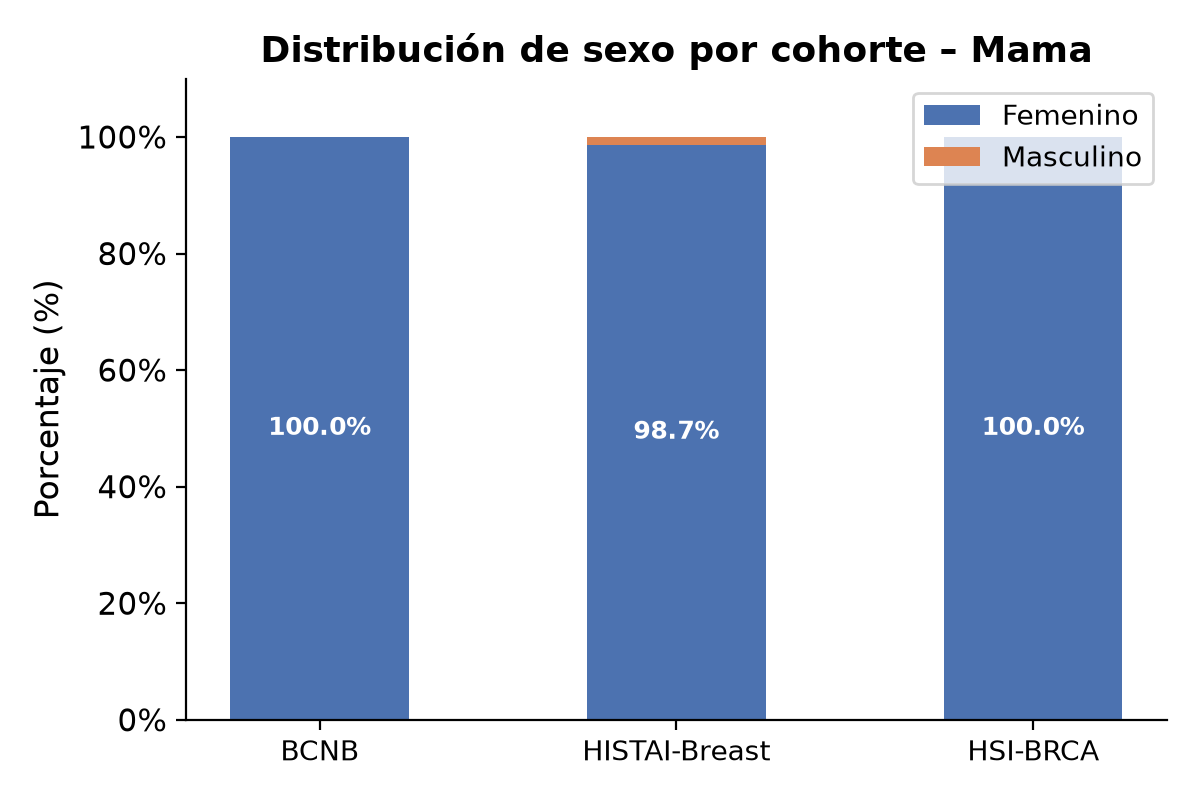
\includegraphics[width=0.65\textwidth]{images/fig_sexo_mama.png}
\caption{Distribución por sexo en los conjuntos de datos de cáncer de mama.}
\label{fig:sexo_mama}
\end{figure}

\begin{figure}[htbp]
\centering
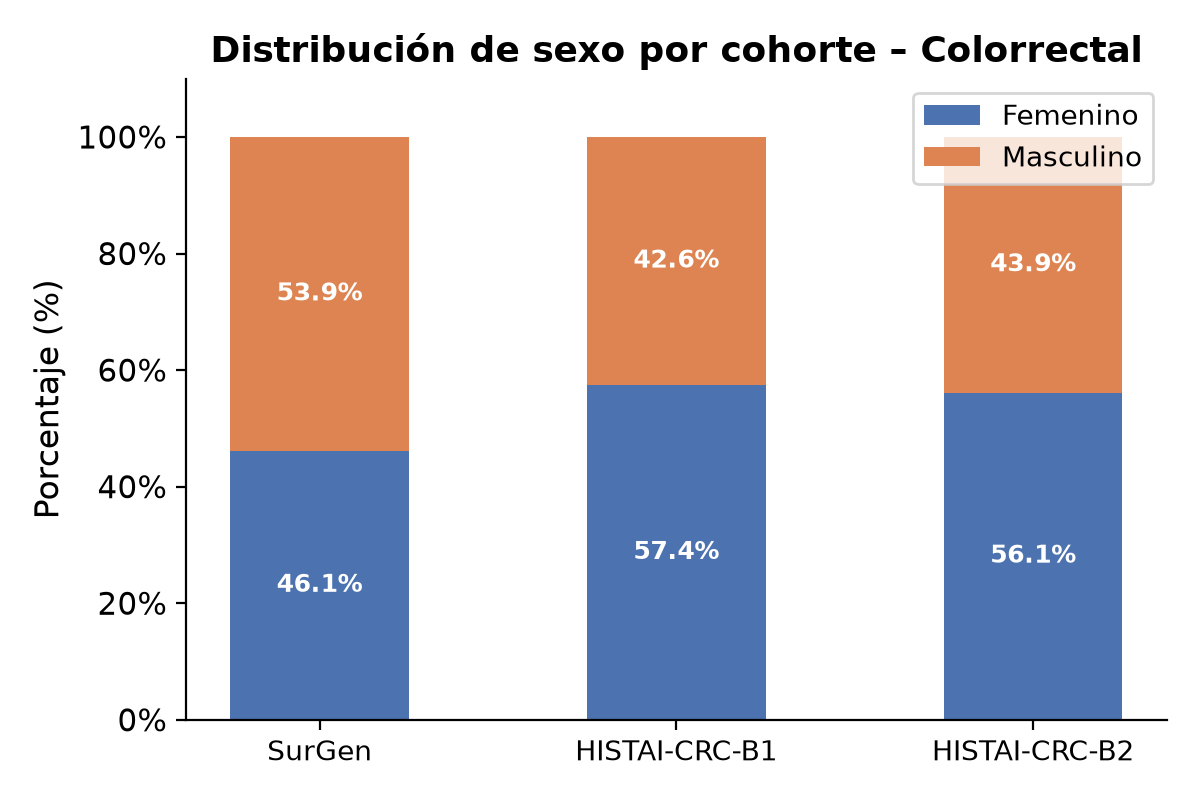
\includegraphics[width=0.65\textwidth]{images/fig_sexo_colorrectal.png}
\caption{Distribución por sexo en los conjuntos de datos de cáncer colorrectal.}
\label{fig:sexo_colorrectal}
\end{figure}

\begin{figure}[htbp]
\centering
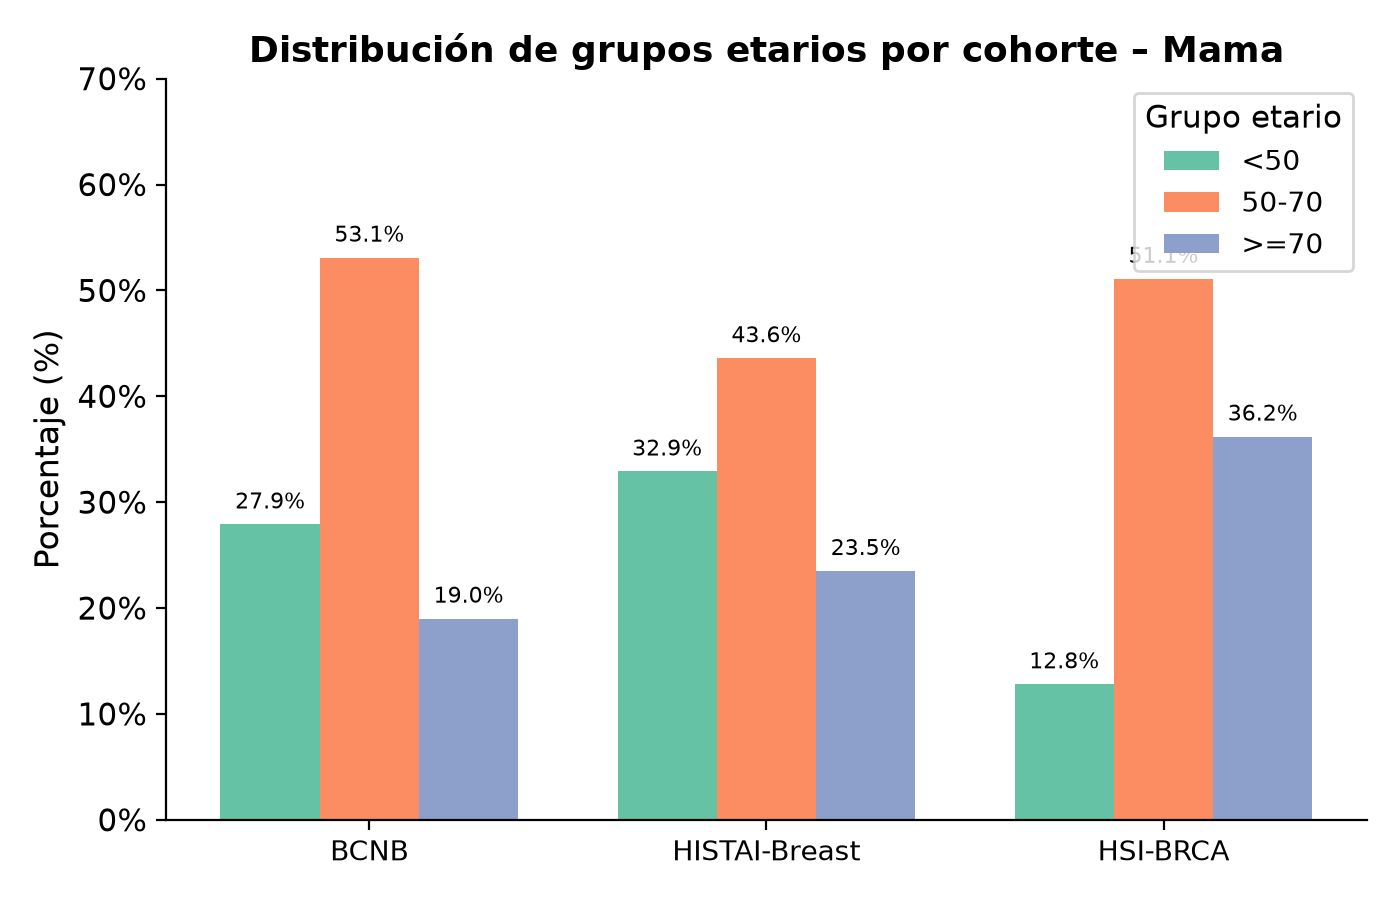
\includegraphics[width=0.65\textwidth]{images/fig_edad_mama.png}
\caption{Distribución por grupos etarios en los conjuntos de datos de cáncer de mama.}
\label{fig:edad_mama}
\end{figure}

\begin{figure}[htbp]
\centering
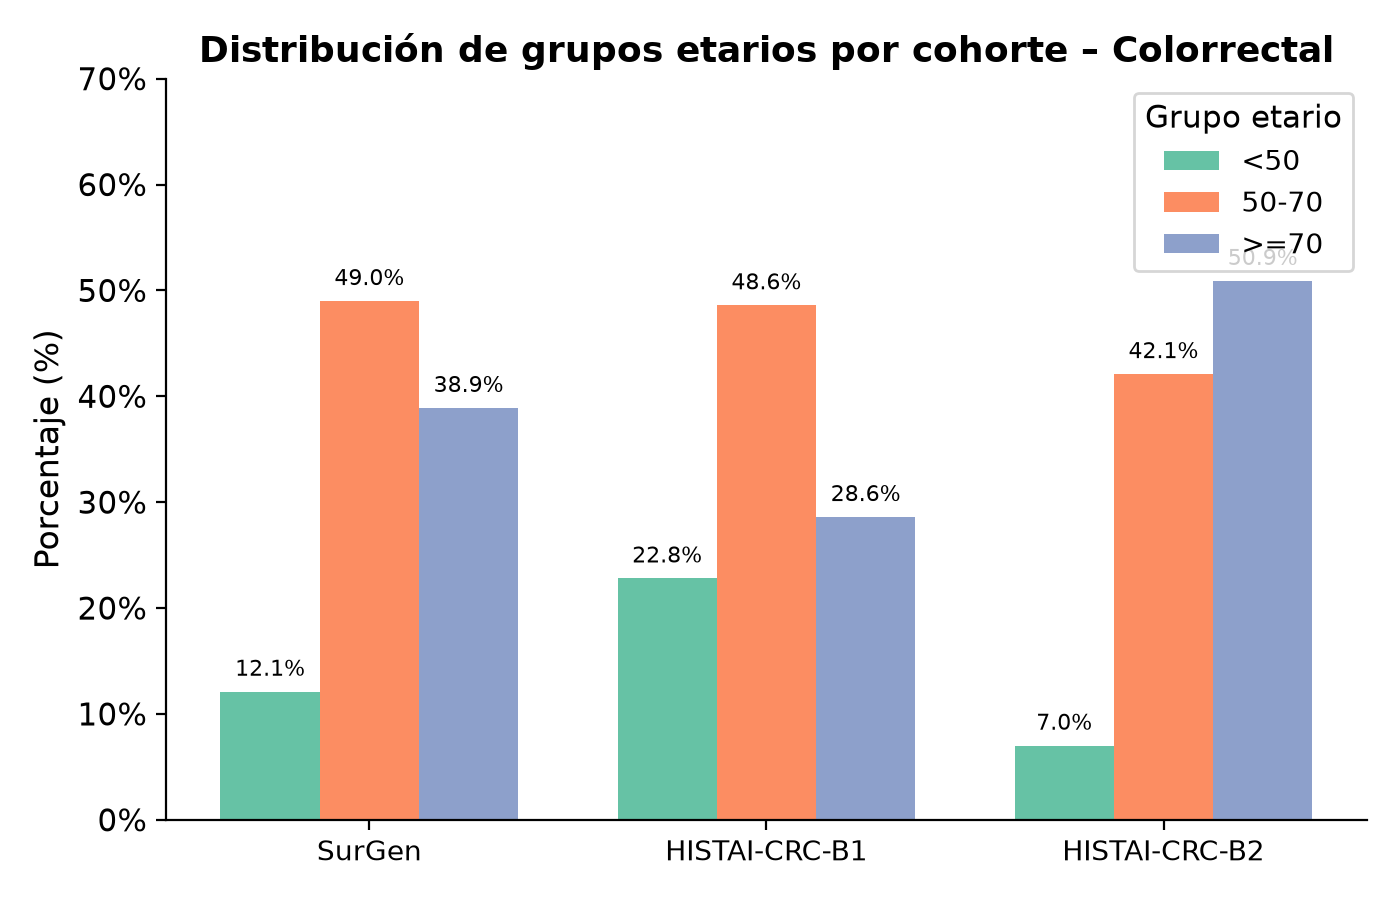
\includegraphics[width=0.65\textwidth]{images/fig_edad_colorrectal.png}
\caption{Distribución por grupos etarios en los conjuntos de datos de cáncer colorrectal.}
\label{fig:edad_colorrectal}
\end{figure}

En mama, las tres cohortes muestran un patrón consistente: distribuciones etarias desplazadas hacia la adultez mayor (medianas entre 57 y 65 años) y una proporción creciente de pacientes de 70 años o más a medida que disminuye el tamaño de la cohorte (19--36\%, Figura~\ref{fig:edad_mama}), lo que constituye una fuente potencial de \textit{bias} de representación. En colorrectal, SurGen e HISTAI-CRC-B2 concentran una proporción considerable de pacientes mayores de 70 años (39\% y 51\%, Figura~\ref{fig:edad_colorrectal}), mientras HISTAI-CRC-B1 es más joven (mediana 63 años); esta heterogeneidad es relevante porque la edad podría correlacionarse con el sitio anatómico y el estado mutacional, introduciendo confusión en análisis comparativos.

\subsection{Distribución de variables objetivo en el dominio de mama}

Se consideraron dos variables objetivo: HER2 (tres clases) y subtipo molecular (cuatro clases), disponibles en las tres cohortes con diferencias de cobertura y forma de reporte (Tabla~\ref{tab:resumen_frecuencias_mama}; cobertura por cohorte en la Tabla~\ref{tab:trazabilidad_mama}).

\subsubsection*{HER2}

La distribución difiere marcadamente entre cohortes: BCNB concentra sus casos entre negativo/bajo y equívoco con baja proporción de positivos; HISTAI-Breast muestra un patrón similar pero con una fracción considerable sin dato recuperable desde texto libre; y HSI-BC presenta fuerte predominio de la categoría negativa, sin equívocos registrados. Estas diferencias podrían reflejar tanto variación real en prevalencia como diferencias en criterios de reporte. En HISTAI-Breast existe además una representación masculina marginal (1,3\%) que, junto con la ausencia total de varianza en sexo en BCNB y HSI-BC, impide el análisis estratificado por sexo en este dominio.

\subsubsection*{Subtipo molecular}

BCNB reporta subtipo para la totalidad de los casos, con predominio de Luminal B y Luminal A. HISTAI-Breast, extraído desde texto libre con 57,2\% de cobertura, muestra un patrón similar pero más concentrado en Luminal B y HER2+. HSI-BC (n=47) presenta predominio de Luminal B con baja representación de HER2+ y Triple negativo, por lo que sus estimaciones deben interpretarse con cautela. En consecuencia, la edad queda como único atributo demográfico utilizable para estratificar comparaciones de \textit{bias} en mama.

\subsection{Distribución de variables objetivo en el dominio colorrectal}

Se consideraron el sitio anatómico del tumor y la lateralidad, armonizados en la curación (Sección~\ref{sec:caracterizacion_datasets}) y reportados en la Tabla~\ref{tab:resumen_frecuencias_colorrectal} (desglose completo en la Tabla~\ref{tab:frecuencias_colorrectal} del Apéndice~\ref{appendix:tablasdatasets}).

\subsubsection*{Sitio anatómico}

Recto, sigmoide y colon derecho concentran la mayoría de los casos en las tres cohortes, con diferencias en la granularidad reportada. Las categorías de baja frecuencia relevantes para \textit{fairness}, rectosigmoide en SurGen (2,3\%) y metástasis hepática en HISTAI-CRC-B1 (2,1\%), concentran pocos casos, implicando mayor variabilidad en esos subgrupos; en HISTAI-CRC-B2 (n=57), cualquier desagregación por sitio debe interpretarse con cautela.

\subsubsection*{Lateralidad}

Definida como simplificación del sitio anatómico (izquierdo, derecho, recto, transverso, rectosigmoide), presenta cobertura parcial (75,0\% en SurGen, 70,0\% en HISTAI-CRC-B1, 80,7\% en HISTAI-CRC-B2). Predominan izquierdo, derecho y recto, mientras transverso y rectosigmoide concentran sistemáticamente menos casos; la lateralidad muestra en general menos desbalance que el sitio anatómico, pero estas categorías de baja frecuencia deben considerarse especialmente en las cohortes más pequeñas.

\subsection{Trazabilidad de muestras a lo largo del pipeline}
\label{sec:trazabilidad_muestras}

Las secciones anteriores describieron las distribuciones demográficas y de variables objetivo sobre la cohorte curada (\textit{post-curation}). Sin embargo, la población efectivamente disponible para una tarea de clasificación puede ser menor, debido a filtros sucesivos: disponibilidad de etiqueta objetivo y completitud de atributos de estratificación (edad, sexo).

Las Tablas~\ref{tab:trazabilidad_mama}~y~\ref{tab:trazabilidad_colorrectal} documentan esta transición para los dominios de mama y colorrectal, respectivamente. Se reportan tres hitos: el tamaño bruto del recurso original (N\textsubscript{raw}), el tamaño después de la curación y armonización (N\textsubscript{curation}), y, para cada variable objetivo, el número de casos de la cohorte analítica final (N\textsubscript{elegible}) y el porcentaje de retención respecto a la cohorte curada. Estos tamaños corresponden exactamente a las poblaciones utilizadas en los experimentos del Capítulo~\ref{cap:evaluacion_modelos}.

\begin{table}[htbp]
\centering
\caption{Trazabilidad de muestras en el dominio de mama.}
\label{tab:trazabilidad_mama}
\footnotesize
\setlength{\tabcolsep}{4pt}
\begin{tabular}{lcccccc}
\toprule
\multirow{2}{*}{\textbf{Dataset}} & \multirow{2}{*}{\textbf{N\textsubscript{raw}}} & \multirow{2}{*}{\textbf{N\textsubscript{cur}}}
  & \multicolumn{2}{c}{\textbf{HER2}} & \multicolumn{2}{c}{\textbf{Subtipo mol.}} \\
\cmidrule(lr){4-5} \cmidrule(lr){6-7}
& & & \textbf{N\textsubscript{ele}} & \textbf{\% ret.} & \textbf{N\textsubscript{ele}} & \textbf{\% ret.} \\
\midrule
BCNB & 1058 & 1058 & 1058 & 100,0 & 1058 & 100,0 \\
HISTAI-Breast & 1489 & 1489 & 870 & 58,4 & 842 & 56,5 \\
HSI-BC & 47 & 47 & 44 & 93,6 & 44 & 93,6 \\
\bottomrule
\end{tabular}
\end{table}

\begin{table}[htbp]
\centering
\caption{Trazabilidad de muestras en el dominio colorrectal.}
\label{tab:trazabilidad_colorrectal}
\footnotesize
\setlength{\tabcolsep}{4pt}
\begin{tabular}{lcccccc}
\toprule
\multirow{2}{*}{\textbf{Dataset}} & \multirow{2}{*}{\textbf{N\textsubscript{raw}}} & \multirow{2}{*}{\textbf{N\textsubscript{cur}}}
  & \multicolumn{2}{c}{\textbf{Sitio}} & \multicolumn{2}{c}{\textbf{Lateralidad}} \\
\cmidrule(lr){4-5} \cmidrule(lr){6-7}
& & & \textbf{N\textsubscript{ele}} & \textbf{\% ret.} & \textbf{N\textsubscript{ele}} & \textbf{\% ret.} \\
\midrule
SurGen & 843 & 841 & 765 & 91,0 & 631 & 75,0 \\
HISTAI-CRC-B1 & 878 & 878 & 878 & 100,0 & 615 & 70,0 \\
HISTAI-CRC-B2 & 57 & 57 & 57 & 100,0 & 46 & 80,7 \\
\bottomrule
\end{tabular}
\end{table}

Como se observa en las tablas, HISTAI-Breast presenta la mayor pérdida de casos en mama (56--58\% de retención), debido a la naturaleza no estructurada de los informes desde los que se extrajeron los biomarcadores. En colorrectal, la lateralidad tiene sistemáticamente menor cobertura que el sitio anatómico, reflejando que no todos los casos con sitio clasificable admiten una lateralidad definida (por ejemplo, sitios inespecíficos o metastásicos). La descripción de las reglas de extracción empleadas, sus criterios de resolución de conflictos y sus errores esperables se presenta en el Apéndice~\ref{appendix:extraccion_histai}.

Esta pérdida puede además alterar la composición demográfica de la población analizable: en HISTAI-Breast, la mediana de edad se desplaza de 58 a 63 años al filtrar por HER2 o subtipo molecular, con menos casos menores de 50 años y más mayores de 70, lo que sugiere que los pacientes mayores tienen mayor probabilidad de contar con biomarcadores extraíbles, un sesgo de selección indirecto por edad en la cohorte elegible.

\subsection{Condiciones de adquisición y potencial de confusión}
\label{sec:adquisicion}

La Tabla~\ref{tab:adquisicion_bias} resume los parámetros de adquisición documentados para cada conjunto de datos seleccionado. Como puede observarse, existe una asociación casi perfecta entre dataset y condiciones de adquisición: todos los casos de un mismo recurso fueron digitalizados con el mismo escáner (o un conjunto acotado de ellos), bajo la misma magnificación y tinción. Esto implica que, en cualquier comparación entre cohortes, la variable \textit{dataset} puede estar confundida con el equipo de digitalización, el protocolo de tinción y el período de recolección.

\begin{table}[htbp]
\centering
\caption{Parámetros de adquisición y riesgo de confusión entre cohortes.}
\label{tab:adquisicion_bias}
\small
\setlength{\tabcolsep}{4pt}
\resizebox{\textwidth}{!}{%
\begin{tabular}{lllll}
\toprule
\textbf{Dataset} & \textbf{Escáner} & \textbf{Magnif.} & \textbf{Tinción} & \textbf{Período} \\
\midrule
BCNB & No reportado & 20x & H\&E & No reportado \\
HISTAI-Breast & Leica Aperio GT450/AT2 & 20x (40x frac.) & H\&E (mayoría) & No reportado \\
HSI-BC & 3DHISTECH P250 Flash III & 20x & H\&E + hiperesp. & 2006--2015 \\
SurGen & ZEISS AxioScan.Z1 & 40x & H\&E & No reportado \\
HISTAI-CRC-B1 & Leica Aperio GT450/AT2 & 20x (40x frac.) & H\&E (mayoría) & No reportado \\
HISTAI-CRC-B2 & Leica Aperio GT450/AT2 & 20x (40x frac.) & H\&E (mayoría) & No reportado \\
\bottomrule
\end{tabular}%
}
\end{table}

Esta confusión tiene implicancias directas para comparaciones \textit{cross-dataset}: una diferencia de desempeño entre BCNB e HISTAI-Breast no podrá atribuirse solo a edad o subtipo molecular, ya que ambas cohortes difieren en escáner, institución y método de determinación de biomarcadores (estructurado vs. extraído de texto libre, con la pérdida selectiva documentada en la Sección~\ref{sec:trazabilidad_muestras}). En colorrectal, aunque las tres cohortes comparten tinción H\&E, persiste diferencia de escáner y magnificación (40x en SurGen vs. 20x en HISTAI); por ello se utilizará la versión a 20x de SurGen, unificando la resolución de trabajo. Esta confusión entre \textit{dataset} y condiciones técnicas corresponde a la principal fuente de sobreestimación de desempeño identificada en patología computacional: cuando \textit{dataset} y centro de origen coinciden, un modelo puede explotar la firma técnica del centro en lugar de la morfología de interés, ventaja que no se transfiere a cohortes externas \parencite{howard2021site}. Este estudio documenta la condición a nivel de metadatos; su efecto sobre el desempeño y las brechas entre subgrupos se evalúa experimentalmente en los Capítulos~\ref{cap:seleccion_modelos}~y~\ref{cap:evaluacion_modelos}.

\subsection{Síntesis de indicadores de \textit{bias} por conjunto de datos}
\label{sec:sintesis_bias}

A modo de síntesis, la Tabla~\ref{tab:matriz_riesgo_unificada} presenta una visión consolidada de los indicadores de \textit{bias} identificados para cada conjunto de datos seleccionado, organizados según los tres mecanismos definidos en la Sección~\ref{sec:marco_bias}: representación, adquisición y documentación/selección. Para cada mecanismo se asigna un nivel de riesgo cualitativo (bajo, medio, alto) basado en la evidencia presentada a lo largo del capítulo, junto con una columna de riesgo global que integra los tres ejes. Los criterios de asignación de cada nivel se detallan en el Apéndice~\ref{appendix:criterios_preseleccion}.

\begin{table}[htbp]
\centering
\caption{Matriz unificada de riesgo de \textit{bias} por conjunto de datos seleccionado.}
\label{tab:matriz_riesgo_unificada}
\small
\setlength{\tabcolsep}{5pt}
\begin{tabular}{lcccc}
\toprule
\textbf{Dataset} &
  \textbf{Representación} &
  \textbf{Adquisición} &
  \textbf{Documentación} &
  \textbf{Riesgo global} \\
\midrule
BCNB &
  \cellcolor{riesgobajo}Bajo &
  \cellcolor{riesgomedio}Medio &
  \cellcolor{riesgobajo}Bajo &
  \cellcolor{riesgobajo}Bajo--Medio \\
HISTAI-Breast &
  \cellcolor{riesgomedio}Medio &
  \cellcolor{riesgomedio}Medio &
  \cellcolor{riesgoalto}Alto &
  \cellcolor{riesgomedio}Medio--Alto \\
HSI-BC &
  \cellcolor{riesgoalto}Alto &
  \cellcolor{riesgobajo}Bajo &
  \cellcolor{riesgobajo}Bajo &
  \cellcolor{riesgoalto}Alto \\
SurGen &
  \cellcolor{riesgobajo}Bajo--Medio &
  \cellcolor{riesgomedio}Medio &
  \cellcolor{riesgomedio}Medio &
  \cellcolor{riesgomedio}Medio \\
HISTAI-CRC-B1 &
  \cellcolor{riesgomedio}Medio &
  \cellcolor{riesgomedio}Medio &
  \cellcolor{riesgomedio}Medio &
  \cellcolor{riesgomedio}Medio \\
HISTAI-CRC-B2 &
  \cellcolor{riesgoalto}Alto &
  \cellcolor{riesgomedio}Medio &
  \cellcolor{riesgobajo}Bajo &
  \cellcolor{riesgoalto}Alto \\
\bottomrule
\end{tabular}
\end{table}

Esto permite identificar patrones transversales: los riesgos más altos se concentran en cohortes de tamaño muy reducido (HSI-BC, HISTAI-CRC-B2), donde la capacidad de realizar análisis estratificados es limitada y cualquier estimación por subgrupo presentará intervalos de confianza amplios. En el extremo opuesto, BCNB destaca como el conjunto de datos con perfil de riesgo más bajo, debido a su tamaño adecuado, completitud casi perfecta y disponibilidad de múltiples variables clínicas estructuradas. HISTAI-Breast presenta un perfil mixto: si bien su tamaño es moderado, el sesgo de selección inducido por la extracción desde texto libre eleva su riesgo de documentación a niveles que deben considerarse al interpretar cualquier análisis basado en esta cohorte.

En cuanto a los mecanismos de \textit{bias}, el de adquisición es el más uniforme entre cohortes: prácticamente todos los conjuntos presentan confusión entre dataset y condiciones técnicas, lo que obliga a considerar este factor en cualquier comparación \textit{cross-dataset}. El \textit{bias} de representación, en cambio, es más variable y depende del dominio: en mama está acotado principalmente a la edad, mientras que en colorrectal permite análisis más ricos al contar con variabilidad en sexo y edad simultáneamente.

\subsection{Implicancias para el análisis de \textit{bias} en etapas posteriores}
\label{sec:implicancias_bias}

El análisis cuantitativo realizado permite extraer varias conclusiones relevantes para la formulación de tareas y la interpretación de resultados en los capítulos siguientes.

En primer lugar, la variable sexo no puede utilizarse como atributo sensible en el dominio de mama, dado que las tres cohortes son abrumadoramente femeninas. Esto no elimina la posibilidad de que existan sesgos de representación por sexo, especialmente si los modelos entrenados exclusivamente con datos femeninos se aplican a pacientes masculinos, pero sí significa que no es posible construir grupos de comparación intra-dataset. En colorrectal, en cambio, el sexo presenta una distribución suficientemente equilibrada como para permitir análisis estratificados, aunque algunas combinaciones de sitio anatómico y sexo presentan tamaños muestrales reducidos.

En segundo lugar, la edad emerge como la variable demográfica más prometedora para el análisis estratificado, al estar disponible con completitud total dentro de la cohorte curada en los seis conjuntos de datos y presentar una distribución con varianza suficiente en todos ellos. Sin embargo, las diferencias en la distribución etaria entre cohortes de un mismo dominio deben ser consideradas al interpretar comparaciones entre conjuntos de datos, ya que podrían reflejar diferencias reales en la población de origen o sesgos de selección en los criterios de inclusión de cada estudio.

En tercer lugar, el análisis de las variables objetivo en cada dominio reveló que ciertas categorías presentan una prevalencia muy baja. Esta condición implica que cualquier análisis estratificado sobre dichos subgrupos producirá estimaciones con intervalos de confianza más amplios y, por lo tanto, con menor capacidad para distinguir una brecha real de una fluctuación muestral. Esta limitación es reconocida en la literatura de \textit{fairness} en imagen médica, donde la escasa representación de determinados subgrupos restringe tanto la fiabilidad de las métricas desagregadas como la aplicabilidad de las técnicas de evaluación de equidad, que en su mayoría requieren subgrupos de tamaño suficiente \parencite{riccilara2022fairness,wastvedt2024small}. El manejo experimental de estas categorías se retoma en el Capítulo~\ref{cap:seleccion_modelos}.

La heterogeneidad observada no invalida el uso de estos conjuntos de datos, sino que define los límites dentro de los cuales pueden realizarse inferencias válidas, límites que se retoman en la formulación experimental de los Capítulos~\ref{cap:seleccion_modelos}~y~\ref{cap:evaluacion_modelos}.

El análisis de sesgo racial/étnico se declara fuera de alcance (ver §\ref{sec:conclusiones_capitulo4}).

\section{Conclusiones del capítulo}
\label{sec:conclusiones_capitulo4}

Este capítulo cumplió el objetivo específico~1 de la tesis: caracterizar los conjuntos de datos disponibles para el estudio de \textit{bias} en patología digital, identificando condiciones de representación, calidad de metadatos y limitaciones de comparabilidad entre cohortes. Los hallazgos obtenidos permiten establecer una base empírica sobre la cual formular tareas de clasificación y diseñar experimentos de evaluación de \textit{fairness} en los capítulos siguientes.

La revisión de nueve recursos públicos iniciales permitió constatar la heterogeneidad estructural que caracteriza al panorama actual de conjuntos de datos de patología digital. Esta heterogeneidad se manifestó en múltiples dimensiones: tamaño de las cohortes (desde 47 hasta más de mil registros), nivel de estructuración de los metadatos, completitud de variables clínicas y parámetros de adquisición. Tras aplicar un proceso sistemático de curación y armonización, se priorizaron seis conjuntos de datos en dos dominios clínicos, mama y colorrectal, seleccionados por presentar variables comparables entre cohortes y viabilidad para formular tareas supervisadas con al menos dos conjuntos por dominio.

La aplicación del marco de \textit{bias} basado en tres mecanismos (representación, adquisición y documentación/selección) reveló que todos los conjuntos de datos presentan algún grado de riesgo potencial, aunque de distinta naturaleza e intensidad. En el dominio de mama, la principal limitación para el análisis de \textit{fairness} es la variabilidad insuficiente de la variable sexo: BCNB y HSI-BC son exclusivamente femeninos, e HISTAI-Breast contiene una fracción masculina marginal (n=20; 1,3\%), insuficiente para un análisis estratificado estable, lo que restringe los atributos sensibles disponibles exclusivamente a la edad. Este hallazgo es consistente con la literatura sobre cáncer de mama, donde la incidencia masculina es sustancialmente menor, y obliga a considerar la edad como el único eje de estratificación demográfica en este dominio. En el dominio colorrectal, en cambio, tanto sexo como edad presentan distribuciones con varianza suficiente, lo que habilita análisis estratificados más ricos.

En cuanto al eje racial/étnico, dos de los recursos revisados (HSI-BC y NDB-UFES) registran información de raza y etnia, pero ninguna de estas cohortes es susceptible de estratificación: NDB-UFES fue excluida en la preselección y HSI-BC (n=47) no proporciona potencia estadística para desagregar. El resto de las cohortes no contienen esta variable, por lo que el sesgo racial/étnico queda fuera de alcance en este diagnóstico.

La trazabilidad de las muestras a lo largo del \textit{pipeline} de datos evidenció que el proceso de extracción de etiquetas no es neutro: en HISTAI-Breast, la necesidad de recuperar biomarcadores desde texto libre introdujo un sesgo de selección etario, desplazando la mediana de edad de 58 a 63 años. Este resultado constituye una advertencia metodológica importante, ya que sugiere que la calidad de la documentación de un conjunto de datos no solo afecta la cantidad de casos utilizables, sino también la composición demográfica de la cohorte analítica. Trabajos recientes han señalado que este tipo de sesgos de documentación suele estar infrarreportado en la literatura de patología computacional \parencite{galanty2024}, lo que refuerza la necesidad de hacerlos explícitos. La metodología de dicha extracción y sus límites de validación se detallan en el Apéndice~\ref{appendix:extraccion_histai}.

En términos de condiciones de adquisición, se documentó una asociación casi perfecta entre conjunto de datos y parámetros técnicos (escáner, magnificación, tinción), lo que implica que cualquier comparación entre cohortes confunde necesariamente diferencias poblacionales con diferencias técnicas. Esta confusión conecta con dos hallazgos distintos de la literatura, que conviene diferenciar. Por una parte, se ha demostrado que el sitio de adquisición puede ser \textbf{inferido} a partir de imágenes histopatológicas digitalizadas, lo que evidencia la existencia de una firma institucional detectable en la propia imagen \parencite{alsaafin2023biased}. Por otra parte, se ha documentado que dichas firmas específicas de sitio \textbf{afectan el desempeño de los modelos}: persisten pese a la normalización de tinción y a las estrategias habituales de aumentación de datos, inducen estimaciones sesgadas de exactitud cuando muestras de un mismo centro aparecen simultáneamente en entrenamiento y validación, y permiten incluso inferir atributos demográficos como la etnia a partir de la procedencia institucional \parencite{howard2021site}. Este segundo fenómeno es el que la literatura denomina \textit{center effect} o \textit{batch effect} propiamente tal.

La distinción es relevante para esta tesis: el presente capítulo documenta únicamente la condición estructural que hace posible ambos fenómenos, la asociación entre cohorte y parámetros técnicos (Sección~\ref{sec:adquisicion}), pero no demuestra que dicha confusión se traduzca efectivamente en un sesgo de desempeño en los modelos evaluados. La existencia de esta confusión no invalida las comparaciones entre cohortes, pero exige interpretar con cautela cualquier diferencia de desempeño \textit{cross-dataset}. La verificación empírica de este riesgo se aborda en el Capítulo~\ref{cap:evaluacion_modelos}, donde se evalúa experimentalmente la magnitud del \textit{center effect} en las comparaciones entre conjuntos de datos.

Los resultados de esta caracterización tienen implicancias directas para el diseño experimental de los capítulos siguientes. En primer lugar, las tareas de clasificación deberán definirse considerando la cobertura real de etiquetas por cohorte, particularmente en HISTAI-Breast donde la extracción desde texto libre limitó la disponibilidad de biomarcadores. En segundo lugar, la comparabilidad semántica de las categorías entre cohortes deberá verificarse explícitamente, especialmente en lo relativo a HER2, donde los criterios de reporte difieren entre conjuntos de datos. En tercer lugar, la evaluación de \textit{fairness} se centrará en la edad como atributo sensible en mama, y en edad y sexo en colorrectal, con la advertencia de que los subgrupos con menor representación muestral producirán estimaciones con intervalos de confianza más amplios, lo que limita la potencia del análisis desagregado \parencite{riccilara2022fairness}.

Lo que este capítulo no permite concluir es igualmente relevante: los indicadores observables aquí identificados no constituyen una prueba de que los modelos entrenados con estos datos exhibirán disparidades de rendimiento. La traducción de estos indicadores en \textit{bias} efectivo depende de la interacción entre las distribuciones de los datos, la arquitectura del modelo y el algoritmo de optimización. Esta distinción entre \textit{bias} potencial en los datos y \textit{bias} efectivo en los modelos es central en la literatura de \textit{fairness} en inteligencia artificial \parencite{mehrabi2021survey}, y será retomada en el Capítulo~\ref{cap:evaluacion_modelos} al contrastar los resultados experimentales con las condiciones de representación documentadas en esta caracterización.
